\documentclass[11pt]{article}
\usepackage[T1]{fontenc}
\usepackage{lmodern}
\usepackage[margin=1in]{geometry}
\usepackage{amsmath,amssymb,amsthm,graphicx}
\usepackage[hidelinks]{hyperref}
\hypersetup{pdftitle={Choosing a coordinate step with one Hessian-vector query},pdfauthor={},pdfsubject={AI-assisted research working paper, pending author review}}
\newtheorem{theorem}{Theorem}
\newtheorem{proposition}[theorem]{Proposition}
\newtheorem{lemma}[theorem]{Lemma}
\newcommand{\R}{\mathbb R}
\title{Choosing a coordinate step with one Hessian-vector query}
\author{}
\date{November 2026}
\begin{document}
\maketitle
\begin{center}\small\emph{AI-assisted working paper. Author verification pending.}\end{center}
\begin{abstract}
Let a two-dimensional quadratic have current gradient \((1,1)\) and
an unknown Hessian \(H\) with \(I\preceq H\preceq\kappa I\). After one
exact Hessian--vector product, a deterministic method chooses a coordinate and
a step size. We measure its decrease relative to the best exact
coordinate step for the actual \(H\). The best worst-case ratio is
\(8(\kappa+1)/(\kappa+3)^2\). For \(\kappa>1\), a query line attains this
value exactly when the magnitudes of its two components are equal.
Such a query identifies a best coordinate and leaves an interval of
possible curvatures along that coordinate. We characterize that interval, give
a finite decision rule for a general reply, and compute the optimum
when the query is restricted to a coordinate axis.
\end{abstract}

\section{The decision and its information}

At the current point, translated to \(0\), write
\[
 f_H(x)=f_0+(1,1)x+\tfrac12 x^\top Hx,\qquad I\preceq H\preceq\kappa I.
\]
A deterministic procedure first chooses a nonzero \(v\) and observes
the vector \(Hv\). It then chooses a coordinate \(j\in\{1,2\}\) and a
step \(\eta\ge0\), and moves to \(-\eta e_j\). The full product \(Hv\) is the only new observation before the
move.
The query direction \(v\) can differ from the executed coordinate.

Write \(q_j=H_{jj}\) and \(m=\min(q_1,q_2)\). The decrease is
\(\Delta_H(j,\eta)=\eta-\eta^2 q_j/2\). The benchmark chooses the
better of the two coordinates and minimizes the quadratic along that
coordinate, so its decrease is \(1/(2m)\). For a feasible \(H\), the relative decrease is
\begin{equation}
 R_H(j,\eta)=m(2\eta-q_j\eta^2).
 \label{eq:payoff}
\end{equation}
For a fixed query \(v\), the policy is a pair of functions
\(j(y)\in\{1,2\}\) and \(\eta(y)\ge0\), where \(y=Hv\). Its
best uniform guarantee and the value of choosing the query are
\[
 V(v)=\sup_{j(\cdot),\eta(\cdot)}
             \ \inf_{I\preceq H\preceq\kappa I}
                 R_H(j(Hv),\eta(Hv)),\qquad
 V_\star=\sup_{v\ne0}V(v).
\]
The posterior is the set of Hessians consistent with the actual
query reply and the spectral bound.

\section{Two sharp scalar calculations}

Normalize \(v\) and choose a unit \(w\perp v\). The reply gives
\(a=v^\top Hv\) and \(b=w^\top Hv\), leaving only \(d=w^\top Hw\)
unknown in the \((v,w)\) frame. If \(1<a<\kappa\), positive
semidefiniteness of \(H-I\) and \(\kappa I-H\) gives the exact interval
\begin{equation}
 d_-=1+\frac{b^2}{a-1},\qquad
 d_+=\kappa-\frac{b^2}{\kappa-a},\qquad d_-\le d\le d_+.
 \label{eq:posterior}
\end{equation}
Indeed each bound is precisely a Schur-complement condition on the
corresponding \(2\times2\) matrix, so their intersection is sufficient.
If \(a=1\) or \(a=\kappa\), the same semidefinite tests force \(b=0\),
and \(d\) may be any number in \([1,\kappa]\). These formulas include
a singleton interval and define the boundary case without division.

\begin{lemma}\label{lem:scalar}
If the same coordinate is best throughout a reply set and its possible
curvatures form \([l,u]\subset(0,\infty)\), its optimal guaranteed
payoff is \(4lu/(l+u)^2\). A step attaining it is \(2/(l+u)\).
\end{lemma}
\begin{proof}
The payoff for this coordinate at curvature \(q\) is
\(2q\eta-q^2\eta^2\), concave as a function of \(q\) for each \(\eta\).
The minimum over the interval is attained at \(l\) or \(u\).
For \(l<u\), the two endpoint parabolas in \(\eta\) meet at the
positive step \(2/(l+u)\), which lies between \(1/u\) and \(1/l\).
To its left the smaller parabola is the one for \(l\) and is
increasing. To its right the smaller parabola is the one for \(u\)
and is decreasing. For \(l=u\), the ordinary exact step is \(1/l\).
Substitution gives the stated value in both cases.
\end{proof}

\section{The optimal query and its worst reply}

\begin{theorem}\label{thm:query}
For \(\kappa>1\),
\[
 V_\star=\frac{8(\kappa+1)}{(\kappa+3)^2},
 \qquad V(v)=V_\star\ \Longleftrightarrow\ |v_1|=|v_2|.
\]
When \(\kappa=1\) the Hessian is known and every query attains one.
\end{theorem}

\begin{proof}
Take \(v=(1,1)^\top/\sqrt2\), \(w=(-1,1)^\top/\sqrt2\).
The two possible coordinate curvatures are
\((a+d)/2-b\) and \((a+d)/2+b\). Choose coordinate \(1\) when
\(b\ge0\) and coordinate \(2\) when \(b<0\). It is best on the
whole posterior and has interval
\[
 l=(a+d_-)/2-|b|,\qquad u=(a+d_+)/2-|b|.
\]
The prior gives \(l\ge1\) and \(u-l\le(\kappa-1)/2\). Thus
\(u/l\le(\kappa+1)/2\). Since \(4t/(1+t)^2\) decreases for
\(t\ge1\), Lemma~\ref{lem:scalar} proves the lower guarantee.
For this query the reply \(Hv=v\) has feasible family
\(H=I+d'ww^\top\), \(0\le d'\le\kappa-1\). The two coordinates
both have interval \([1,(\kappa+1)/2]\), so the guarantee is attained
as a worst payoff on this reply.

For the converse write \(v=(c,s)^\top\) with \(c\ge s\ge0\) and
\(c^2+s^2=1\). This entails no loss of generality. Signed coordinate
permutations conjugate the Hessian prior and the query replies, and
they preserve or relabel diagonal curvatures. The specified gradient
can be kept fixed because the payoff \eqref{eq:payoff} depends on the
Hessian only through its diagonal. Let \(w=(-s,c)^\top\), and define
\[
 \delta=\frac{\kappa-1}{c(c+s)},\quad
 \lambda=1+\delta(c^2-s^2),\quad
 H_L=\begin{pmatrix}\lambda&0\\0&1\end{pmatrix},\quad
 H_U=H_L+\delta ww^\top .
\]
Both give the same query reply since \(w^\top v=0\). The diagonal
entry \(\lambda=1+(\kappa-1)(c-s)/c\) lies in \([1,\kappa]\).
The two diagonal entries of \(H_U\) are
\(u=1+\delta c^2\), and its off-diagonal is \(-\delta cs\).
Its largest eigenvalue is \(u+\delta cs=\kappa\). The smallest is
\(1+(\kappa-1)(c-s)/(c+s)\ge1\). Both Hessians are feasible.

Coordinate \(2\) is a best choice for both and weakly dominates
coordinate \(1\) at any fixed step, because its curvature is weakly
smaller. At the two indistinguishable endpoints its curvature is \(1\)
and \(u\), respectively. The calculation in Lemma~\ref{lem:scalar}
bounds the guaranteed payoff by \(4u/(1+u)^2\). Here
\[
 u=1+\frac{(\kappa-1)c}{c+s}\ \ge\ \frac{\kappa+1}{2},
\]
with a strict inequality for \(c>s\). This gives the stated optimum
and its strict characterization. The signed balanced lines attain it
by the same symmetry as above.
\end{proof}

On the reply just constructed, the whole feasible set is
\(H_L+tww^\top\), \(0\le t\le\delta\). To see this, any symmetric
matrix with the reply differs by a multiple of \(ww^\top\). Its
second diagonal forces \(t\ge0\). The vector \((1,-1)^\top\) has
Rayleigh value \(\kappa\) at \(H_U\) and is not orthogonal to \(w\);
the upper spectral bound therefore forces \(t\le\delta\).
Convexity of the prior gives feasibility for the entire segment.
There the difference between the first and second diagonal entries
is \((\delta-t)(c^2-s^2)\ge0\). The hard reply fixes a best coordinate
and leaves uncertainty about how far to move.

\section{A rule for any query reply}

For a fixed \(v=(c,s)\) and \(w=(-s,c)\), write the candidate curvatures as
\[
 q_1(d)=ac^2-2bcs+ds^2,\qquad
 q_2(d)=as^2+2bcs+dc^2.
\]
Let \(l_j=q_j(d_-)\), \(u_j=q_j(d_+)\) and let
\(m_L=\min_jl_j\), \(m_U=\min_ju_j\). A step larger than \(2/u_j\)
gives a negative payoff at \(d_+\), while step zero guarantees zero.
For \(0\le\eta\le2/u_j\), the factor \(2\eta-q_j(d)\eta^2\)
is nonnegative throughout the posterior. The payoff at \(d\) is
therefore the minimum over \(i=1,2\) of
\(q_i(d)(2\eta-q_j(d)\eta^2)\). Each expression is concave in \(d\),
since the slopes of both curvatures are nonnegative. Their minimum
is concave, and hence its minimum over the interval is at an endpoint.
The exact conditional guarantee for chosen \(j,\eta\) is
\begin{equation}
 \min\{m_L(2\eta-l_j\eta^2),\,m_U(2\eta-u_j\eta^2)\}.
 \label{eq:conditional}
\end{equation}
For each \(j\), maximize this over the domain endpoints, the
feasible vertices \(1/l_j\) and \(1/u_j\), and the feasible positive
intersection
\[
 \frac{2(m_U-m_L)}{m_Uu_j-m_Ll_j}
\]
when its denominator is positive. These are all possibilities because
between intersections the objective is one of two concave parabolas.
If the denominator is zero, the two parabolas coincide by positivity
and endpoint monotonicity. Take the better of the two coordinate
values. This is a conditional calculation in terms of the actual
reply. The pair in Theorem~\ref{thm:query} gives an upper bound for
each unbalanced orientation, but it need not be a worst reply for
that orientation.

\section{The exact value of an axis query}

\begin{proposition}\label{prop:axis}
Suppose \(\kappa>1\), let \(\varphi=(1+\sqrt5)/2\), and fix \(v=e_1\).
For \(1<\kappa\le\varphi^2\), \(V(e_1)=1/\sqrt\kappa\).
For \(\kappa>\varphi^2\), \(V(e_1)=1/a_\kappa\), where
\(a_\kappa\) is the unique root in \((2-1/\kappa,\kappa)\) of
\[
 4a^2(a-1)(\kappa-1)=(\kappa a-1)^2 .
\]
\end{proposition}

\begin{proof}
The reply specifies \(a=H_{11}\) and the off-diagonal. For a fixed
\(a\), the widest compatible interval for \(d=H_{22}\) occurs when the
off-diagonal is zero and is then exactly \([1,\kappa]\).
The payoff depends only on \(a,d\). A strategy valid for that interval
is valid for all smaller reply sets with the same \(a\), and the
diagonal family itself is feasible. It suffices to solve this
one-dimensional decision for each \(a\in[1,\kappa]\).

For coordinate \(1\), the choice \(1/a\) is pointwise optimal.
The worst value is \(1/a\), attained at \(d=1\). For coordinate \(2\),
\eqref{eq:conditional} gives
\[
 w_\kappa(a)=\max_{0\le\eta\le2/\kappa}
     \min\{2\eta-\eta^2,\ a(2\eta-\kappa\eta^2)\}.
\]
Set \(a_0=2-1/\kappa\). If \(a\le a_0\), evaluate at the vertex
\(\eta=1/\kappa\) of the second parabola. Its value \(a/\kappa\)
is at most the first parabola there, yielding
\(w_\kappa(a)=a/\kappa\). If \(a>a_0\), the positive intersection is
\(\eta_\star=2(a-1)/(\kappa a-1)\). It lies strictly to the right
of \(1/\kappa\) and at or to the left of \(1\) and \(2/\kappa\).
The latter inequalities follow from \(a\le\kappa\) and
\(\kappa(2-\kappa)\le1\). To its left the minimum is the increasing
first parabola. To its right the second parabola is decreasing.
Consequently
\[
 w_\kappa(a)=
 \begin{cases}
 a/\kappa,&1\le a\le a_0,\\
 4a(a-1)(\kappa-1)/(\kappa a-1)^2,&a_0<a\le\kappa .
 \end{cases}
\]
This function is strictly increasing. On the second branch
\(\eta_\star\) increases with \(a\) and \(2\eta_\star-\eta_\star^2\)
increases for \(\eta_\star<1\). At \(a=1\) the value \(1/a\) exceeds
\(w_\kappa(a)\), and at \(a=\kappa\) it is smaller, because the
second branch is strictly increasing from \(a_0/\kappa>1/\kappa\).
Thus the optimum across replies,
\(\min_{a\in[1,\kappa]}\max\{1/a,w_\kappa(a)\}\), occurs at the unique
crossing. On the first branch the crossing is \(a=\sqrt\kappa\), valid
exactly when \(\sqrt\kappa\le a_0\), or \(\kappa\le\varphi^2\):
for \(t=\sqrt\kappa>1\) this inequality is
\((t-1)(t^2-t-1)\le0\). Otherwise equating the second branch to \(1/a\)
gives the stated equation on \((a_0,\kappa)\).
\end{proof}

For instance, at \(\kappa=2\) an axis query guarantees \(1/\sqrt2\).
The balanced guarantee is \(24/25\). The all-orientation upper bound
from the pair in Theorem~\ref{thm:query} is \(8/9\) at this axis.
This example makes the distinction between a useful orientation bound
and the exact value of a fixed orientation concrete.

\begin{figure}[!h]
 \centering
 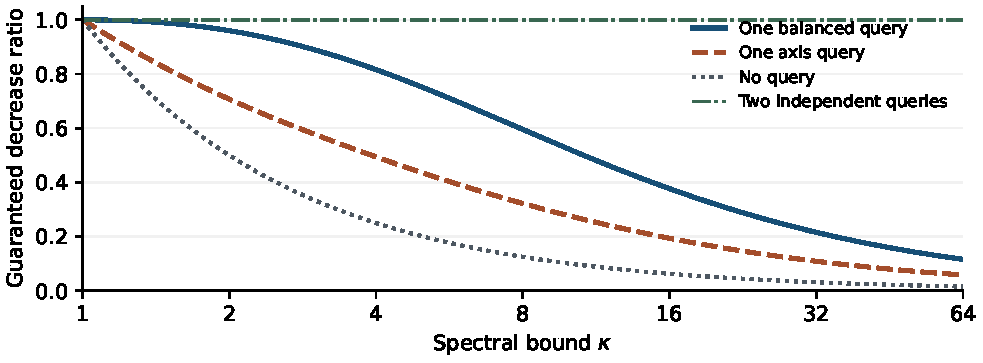
\includegraphics[width=.86\linewidth]{query-values.pdf}
 \caption{Worst-case decrease relative to the best exact coordinate
 line search. The axis curve uses Proposition~\ref{prop:axis}; its
 implicit branch is evaluated by bisection.}
 \label{fig:guarantees}
\end{figure}

\clearpage
\section{What the query reveals}

With no query a deterministic coordinate step has value \(1/\kappa\).
For any chosen coordinate the adversary can give it curvature
\(\kappa\) and the other curvature \(1\), and maximizing the resulting
\(2\eta-\kappa\eta^2\) yields \(1/\kappa\). The step \(1/\kappa\)
guarantees that value by \(m\ge1\) and \(q_j\le\kappa\).
With two independent queries the Hessian is known and the value is one.
Figure~\ref{fig:guarantees} compares these cases with the balanced and
axis rules proved above.



A balanced query reveals the contrast \(H_{11}-H_{22}\).
An unbalanced query with unit perpendicular \(w\) cannot always
identify the best coordinate: the feasible Hessians
\((\kappa+1)I/2\pm\varepsilon ww^\top\) give the same reply and
opposite nonzero diagonal contrasts for small \(\varepsilon>0\).
Identifying the coordinate is a linear decision about the
contrast of two costs, as in \cite{informativeness}. The chosen
coordinate's curvature also sets the step length, so the guaranteed
decrease requires the scalar calculation in Lemma~\ref{lem:scalar}. For the maximum posterior
curvature width over the entire unit circle, every unit query has
the same worst width \(\kappa-1\). Restricting the width to the two
executed coordinates changes it to
\((\kappa-1)\max(v_1^2,v_2^2)\), which is minimized by balanced
queries. Both width formulas follow because two compatible
Hessians differ by a multiple of \(ww^\top\), and the reply
\(Hv=v\) attains the full scalar range of the multiple.

These guarantees are for a deterministic one-step coordinate decision
with two equal directional derivatives. They compare the achieved
decrease with the best exact coordinate line search on the same
quadratic. Randomized queries, general executed directions and
comparisons with a multi-step BB run require different decision
problems.

\paragraph{Status and AI disclosure.}
This AI-assisted working paper is based on a previously developed
coordinate-query derivation and is pending human author review.
The companion source records exact rational checks of representative
matrices, endpoint payoffs and tests on either side of an axis-query crossing. The general
minimax and uniqueness arguments are supplied in the mathematical
proofs above.

\begin{thebibliography}{9}
\bibitem{informativeness}
O. Bennouna, A. Bennouna, S. Amin, and A. Ozdaglar,
What data enables optimal decisions? An exact characterization for
linear optimization, \emph{NeurIPS}, 2025.
\href{https://arxiv.org/abs/2505.21692}{arXiv:2505.21692}.
See also \emph{Data informativeness in linear optimization under
uncertainty}, \href{https://arxiv.org/abs/2602.15365}{arXiv:2602.15365}.
\end{thebibliography}
\end{document}
